% !TEX root = ../main.tex

\section{Introduction}
In this report, we attempt to validate the experimental results of ``BBR:
Congestion-based Congestion Control''~\cite{cardwell2016bbr}. We start
by looking at the goals, motivations and results from the BBR
\cite{cardwell2016bbr} paper.

\para{Goals}
What was the original paper trying to solve?

The original paper was trying to find a congestion control approach
that would stay as close as possible to optimal network operating point
in various network conditions. The network link is operating at the optimal
point when bandwidth utilization is maximized and latency is minimized.

\para{Motivation}
Why is the problem important/interesting?

This is importannt problem to tackle because traditional congestion control
algorithms such as CUBIC have a tough time operating efficiently when there
is non-negligible packet loss on the packet. This limitation comes from the
CUBIC's use of packet loss as a signal for congestion, which can unnecesarily
hinder throughput leading to poor performance.


\para{Results}
What did the original authors find?

The BBR paper descibes a new form of congestion control that is based on actual
congestion going in the network. The insight from the authors is that their
approach estimates bottleneck bandwidth and then bottleneck latency in succession
so as to be able to get as close as possible to the ideal operating point of
maximum bandwidth and minimal latency. The paper had severals findings.


The first finding is that BBR can quickly adopt to changes in bottleneck link bandwidth.
During operating, BBR spends most of its time continously probing if more bandwidth has
become available. Figure~\ref{fig:bbr3} shows BBR reatcing to a 2x increase and a 2x decrease
to bottleneck bandwidth within about 2 seconds.

The second finding is that BBR is able to avoid bloating router buffers unnecesarilly and thus
it is able to keep RTT at a minimum value. This is contrast to CUBIC which continues to bloat
a router's buffer until it observes a packet loss event from overflowing the router buffer.
Figure~\ref{fig:bbr5} shows CUBIC and BBR behave in this regard.

The third and perhaps most important finding is that BBR outperforms CUBIC for non-negligible loss rates.
Figure~\ref{fig:bbr8} shows a graph showing the performance comparison between BBR and CUBIC
for varying loss rates.

The authors report that Google has had a very good experience deploying BBR on B4. B4 is Google  data center to
data center high-speed Wide Area Network and it's built primarily from commodity switches that have shallow/small
memory buffers. The limited amount of buffering means that there is the occasional packet loss when there is a
a burst of incoming packets that arrive at the same time. After switching to BBR from CUBIC, Google saw throughput
improvements ranging from 2x to 25x.

Lastly, the authors do acknowledge that there is still work to be done in terms of how BBR interoperates
with existing loss-based congestion controls algorithms such as CUBIC. In cases where routers have large buffers,
CUBIC senders can drown out BBR. Gracefully mitigating this is an onging area of research.



\begin{figure}[h]
  \centering
  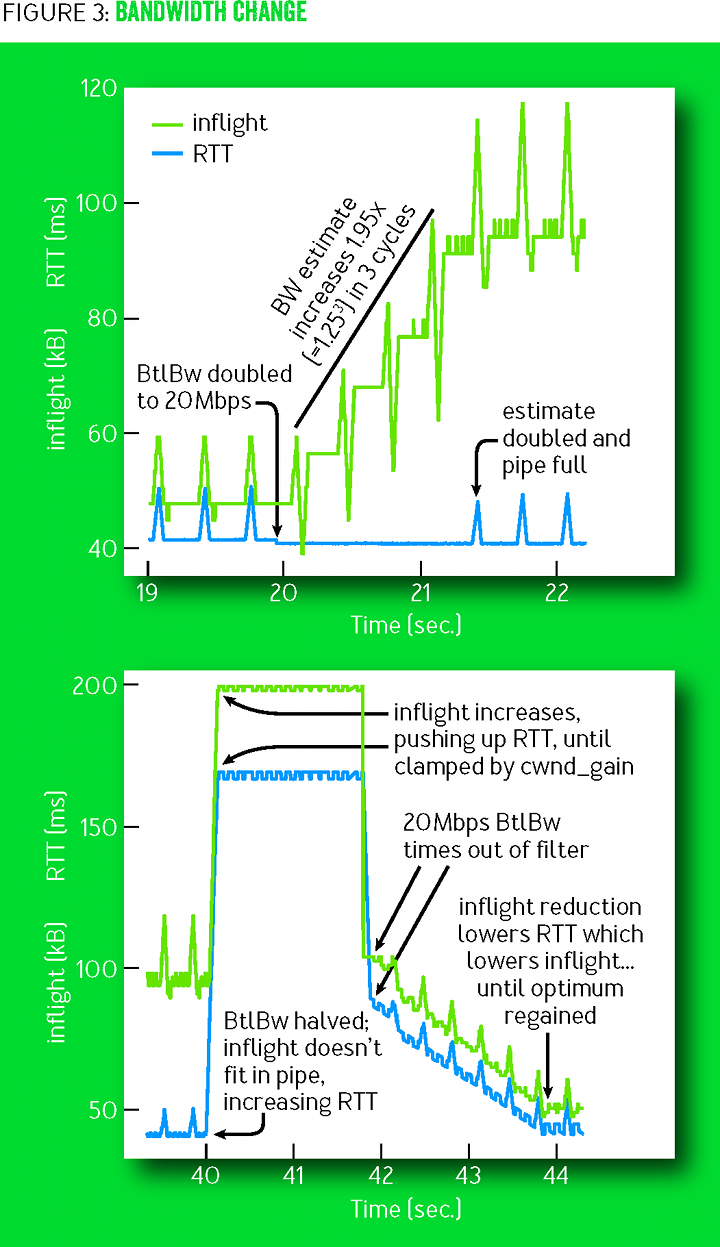
\includegraphics[height=7cm]{./img/bbr_fig3.png}
  \caption{BBR converges to new bottleneck bandwidth at exponential rate.}
  \label{fig:bbr3}
\end{figure}


\begin{figure}[h]
  \centering
  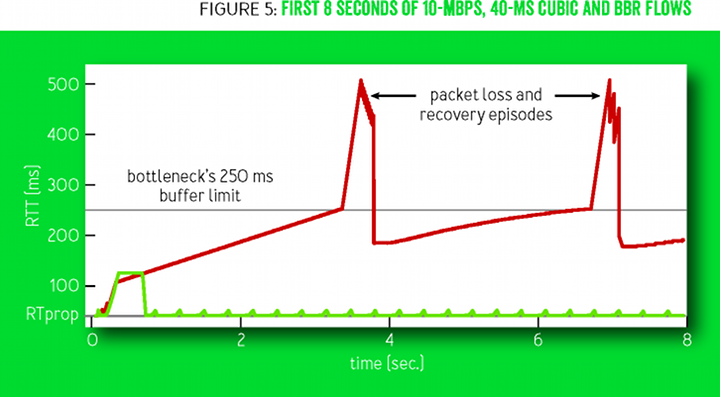
\includegraphics[height=7cm]{./img/bbr_fig5.png}
  \caption{BBR avoids bloating router buffer unlike CUBIC.}
  \label{fig:bbr5}
\end{figure}



\begin{figure}[h]
  \centering
  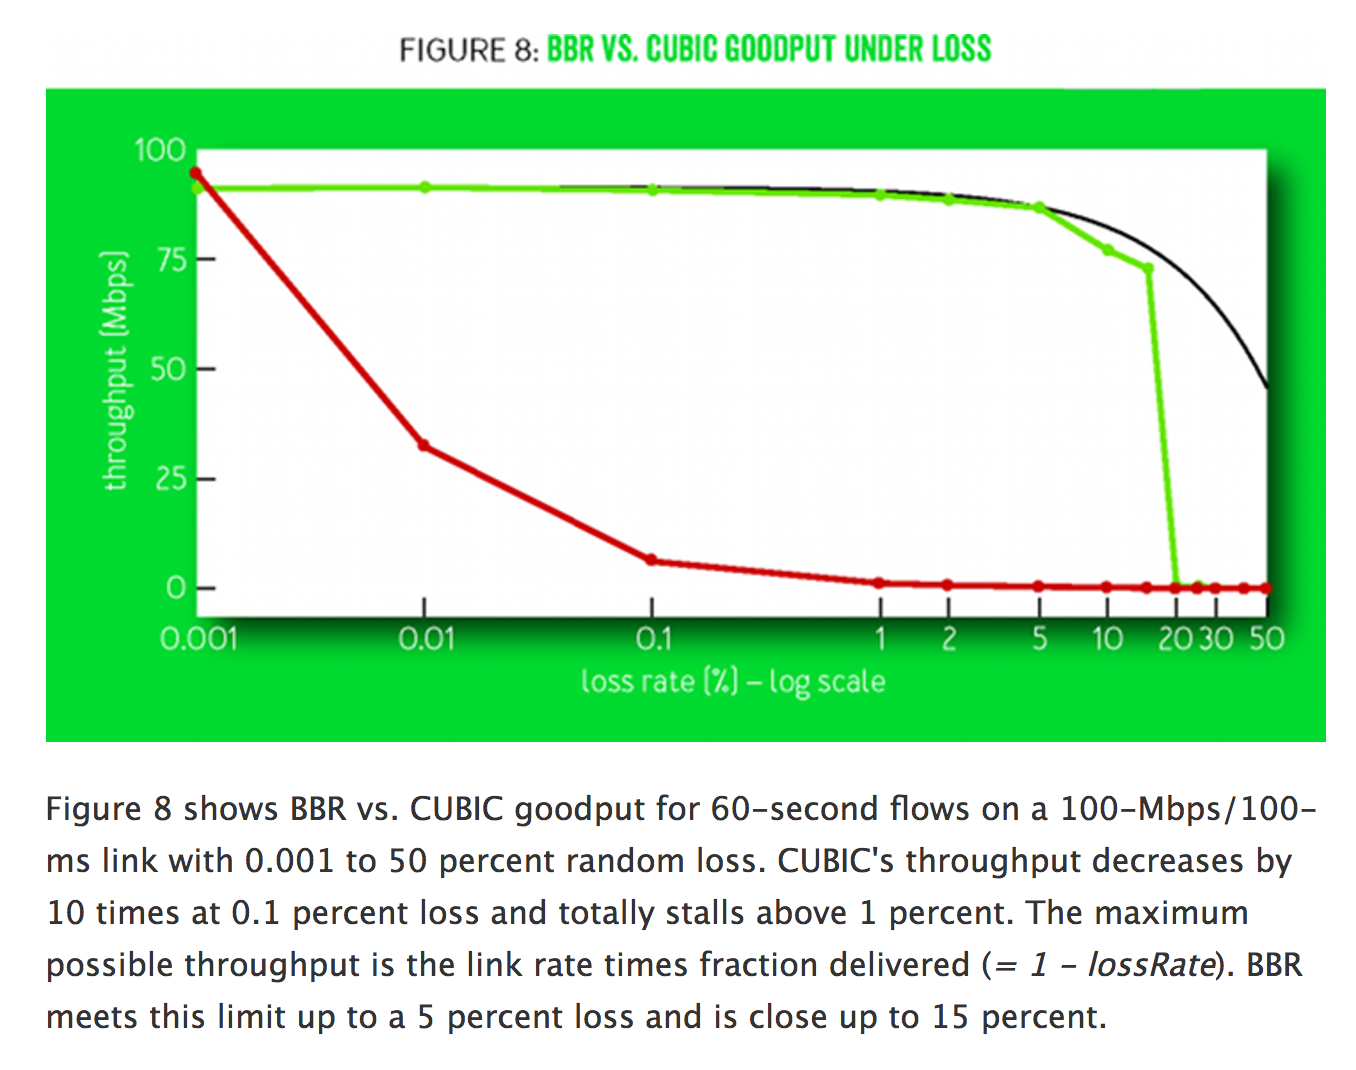
\includegraphics[height=7cm]{./img/bbr_fig8.png}
  \caption{Throughput vs loss rate comparing CUBIC vs BBR.}
  \label{fig:bbr8}
\end{figure}
